\chapter{Evaluation}
\label{chap:evaluation}

This chapter evaluates the performance of our Tsetlin Machine implementation. To ensure comparability with existing research, we focus on standard datasets used in the original studies~\cite{granmo2021tsetlinmachinegame} (e.g. the Noisy-XOR problem). In addition, we provide a baseline comparison with established machine learning models from the Scikit-learn~\cite{scikit-learn} library.

\paragraph{Environment}
The evaluation was conducted in two distinct environments to cover different use cases:
\begin{compactitem}
    \item \textbf{Host (PC)}: Windows 11 25H2 (WSL2 6.6.87.2) on an x86\_64 AMD Ryzen 9 7900X, running Python 3.13.9 and Scikit-learn 1.6.1~\cite{scikit-learn}.
    \item \textbf{Embedded}: Raspberry Pi Pico utilizing the Pi Pico SDK V2.2.0~\cite{pico-sdk}.
\end{compactitem}

\paragraph{Tsetlin Machine default parameters}
The default hyperparameters established during the development of our \texttt{C Tsetlin} classifier are used as a baseline. They are detailed in Table~\ref{tab:tm-default-params}. These values were maintained across all Tsetlin Machine models to ensure a fair comparison. However, we observed that the \GreenTsetlinName library uses undocumented optimizations, such as the \texttt{literal\_budget} parameter, which complicates the verification of its underlying model structure.

\begin{table}[!htbp]
\centering
\caption[Tsetlin Machine default parameters]{Standardized default hyperparameters across Tsetlin Machine implementations, established using the \texttt{C Tsetlin} classifier baseline\label{tab:tm-default-params}.}
\begin{tabularx}{\textwidth}{@{}l L@{}} \toprule
    \textbf{Model} & \textbf{Default Parameters} \\ \midrule \midrule
    \texttt{C Tsetlin} & \texttt{threshold=1000, num\_clauses=1000, max\_state=127, min\_state=-127, boost\_true\_positive\_feedback=False, s=3.0, epochs=10} \\ \midrule
    \texttt{C Tsetlin Sparse} & \texttt{threshold=1000, num\_clauses=1000, max\_state=127, min\_state=-127, boost\_true\_positive\_feedback=False, s=3.0, epochs=10} \\ \midrule
    \texttt{Green Tsetlin} & \texttt{threshold=1000, n\_clauses=1000, boost\_true\_positives=False, s=3.0, n\_epochs=10, literal\_budget=None} \\ \midrule
    \texttt{Green Tsetlin Sparse} & \texttt{threshold=1000, n\_clauses=1000, boost\_true\_positives=False, s=3.0, n\_epochs=10, literal\_budget=None, dynamic\_AL=True, lower\_ta\_threshold=-40, active\_literals\_size=100, clause\_size=50} \\ \bottomrule
\end{tabularx}
\end{table}

\paragraph{Metrics}
The benchmarks on the host were executed via Jupyter Notebooks using our Python bindings. This enabled a direct performance comparison against Scikit-learn models and the \GreenTsetlinName library. We tracked the following metrics: Accuracy on Training Dataset, Accuracy on Testing Dataset, Training Time, Prediction Time on Training Dataset, Prediction Time on Testing Dataset, Estimated Model Size. The model size for TM-based models is estimated based on the internal data structures, while Scikit-learn models use Python \texttt{pickle} exports. Consequently, both these figures and the run times should be compared with caution due to implementation differences.

\paragraph{Embedded hardware}
In order to assess the behavior of our implementation, we analyzed how specific hyperparameters, epoch counts, and batch numbers influence model learning. As a final proof of concept, we deployed a minimal Noisy-XOR example on the Raspberry Pi Pico using only the core C library, demonstrating the feasibility of application on resource-constrained hardware.

\clearpage
\section{Noisy-XOR Dataset}
In the evaluation of our implementation, we first utilized the Noisy-XOR problem, a common benchmark for Tsetlin Machines introduced in~\cite{granmo2021tsetlinmachinegame}. This problem is often challenging for many machine learning models because the XOR relation is non-linearly separable and its complexity increases when noise is added.

\paragraph{Dataset and problem representation}
The dataset consists of $1000$ randomly generated samples with $16$ features. The true target label was determined by the XOR sum of only the first two features (e.g. $x: [0,1,0,\dots,0], y: 1$), while the remaining $14$ features are random noise. To simulate real-world conditions, a noise level of $10\%$ was introduced by flipping the target bit.

\paragraph{Preprocessing and input format}
The final dataset was divided into a training set ($80\%$) and a testing set ($20\%$), maintaining class proportions of approximately $53\%$ for $\text{Class } 0$ and $47\%$ for $\text{Class } 1$. Because TMs operate using Boolean algebra and the generated data was already binary, no additional preprocessing was required, and the raw bits were passed directly to the models.

\paragraph{Model hyperparameters}
We aimed to evaluate the base models using the default parameters while tuning specific configurations via \texttt{GridSearchCV}. The parameters used are detailed in Table~\ref{tab:noisy-xor-params}. For this problem, which features only $16$ binary inputs, \texttt{GridSearchCV} determined that $64$ clauses were sufficient for optimal performance.

\paragraph{Results and comparison}
The results in Table~\ref{tab:noisy-xor-results} demonstrate that our \texttt{C Tsetlin} classifier is highly competitive, matching the accuracy of established machine learning models and performing closely to the \texttt{Green Tsetlin} classifier. Due to the $10\%$ added noise, we expect model accuracy to cap at $0.9$ on the training dataset unless overfitting occurs (as seen in the \texttt{Random Forest} and \texttt{MLP} models). On the testing dataset, our implementation tied for the best result alongside \texttt{SVC} and \texttt{Green Tsetlin} classifier. Slightly longer training and prediction time are likely the result of \LibraryName not implementing vectorization, as decided in the design (see Section~\ref{sec:design}). Furthermore, the version optimized via \texttt{GridSearchCV} is significantly smaller and faster than the version using default parameters, highlighting the importance of parameter tuning.

\begin{table}[!htbp]
\centering
\caption[Noisy-XOR hyperparameters]{Hyperparameters and \texttt{GridSearchCV} search spaces for the Noisy-XOR dataset. The table lists only parameters that differ from model defaults; for \texttt{GridSearchCV} the best-performing configuration is indicated in \texttt{\textbf{\underline{bold}}}\label{tab:noisy-xor-params}.}
\begin{tabularx}{\textwidth}{@{}l L@{}} \toprule
    \textbf{Model} & \textbf{Modified Parameters} \\ \midrule \midrule
    \texttt{Logistic Regression} & \texttt{max\_iter=1000} \\ \midrule
    \texttt{Decision Tree} & \texttt{---} \\ \midrule
    \texttt{Random Forest} & \texttt{---} \\ \midrule
    \texttt{MLP} & \texttt{max\_iter=1000, solver="lbfgs"} \\ \midrule
    \texttt{SVC} & \texttt{---} \\ \midrule
    \texttt{Linear SVC} & \texttt{dual="auto"} \\ \midrule
    \texttt{K-Nearest Neighbors} & \texttt{---} \\ \midrule
    \texttt{Gaussian Naive Bayes} & \texttt{---} \\ \midrule
    \texttt{Gradient Boosting} & \texttt{---} \\ \midrule
    \texttt{LightGBM} & \texttt{---} \\ \midrule
    \texttt{GridSearch Random Forest} & \texttt{n\_estimators: [\textbf{\underline{50}}, 100, 200], max\_depth: [\textbf{\underline{None}}, 10, 20, 30], min\_samples\_split: [2, 5, \textbf{\underline{10}}]} \\ \midrule
    \texttt{GridSearch MLP} & \texttt{hidden\_layer\_sizes: [(50,), \textbf{\underline{(100,)}}, (50, 50)], activation: [\textbf{\underline{"relu"}}, "tanh"], alpha: [0.0001, 0.001, \textbf{\underline{0.01}}]} \\ \midrule \midrule
    \texttt{Green Tsetlin} & \texttt{---} \\ \midrule
    \texttt{Green Tsetlin Sparse} & \texttt{---} \\ \midrule
    \texttt{C Tsetlin} & \texttt{---} \\ \midrule
    \texttt{GridSearch C Tsetlin} & \texttt{boost\_true\_positive\_feedback: [\textbf{\underline{False}}, True], num\_clauses: [\textbf{\underline{64}}, 125, 500], s: [\textbf{\underline{3}}, 9]} \\ \midrule
    \texttt{C Tsetlin Sparse} & \texttt{---} \\ \midrule
    \texttt{GridSearch C Tsetlin Sparse} & \texttt{boost\_true\_positive\_feedback: [\textbf{\underline{False}}, True], num\_clauses: [\textbf{\underline{64}}, 125, 500], s: [\textbf{\underline{3}}, 9]} \\ \bottomrule
\end{tabularx}
\end{table}

\begin{table}[!htbp]
\centering
\setlength{\tabcolsep}{4pt}
\renewcommand{\arraystretch}{0.85}
\setlength{\aboverulesep}{2pt}
\setlength{\belowrulesep}{2pt}
\caption[Noisy-XOR benchmark results]{Benchmark results for the Noisy-XOR dataset (evaluated on the Host (PC) environment). Model sizes are estimated based on internal data structures for Tsetlin-based models and via \texttt{pickle} exports for standard models, requiring caution when comparing directly. The best results are indicated in \texttt{\textbf{\underline{bold}}}\label{tab:noisy-xor-results}.}
\begin{tabularx}{\textwidth}{@{}l c c c c c r@{}} \toprule
    \textbf{\makecell[l]{Model}} & \textbf{\makecell[l]{Train\\Acc.}} & \textbf{\makecell[l]{Test\\Acc.}} & \textbf{\makecell[l]{Train\\Time (s)}} & \textbf{\makecell[l]{Train\\Pred.\\Time (s)}} & \textbf{\makecell[l]{Test\\Pred.\\Time (s)}} & \textbf{\makecell[l]{Model\\Size (B)}} \\ \midrule
    \texttt{\makecell[l]{Logistic Regression}} & \texttt{0.5487} & \texttt{0.4750} & \texttt{0.0028} & \texttt{0.0005} & \texttt{\textbf{\underline{0.0003}}} & \texttt{1,122} \\
    \texttt{\makecell[l]{Decision Tree}} & \texttt{\textbf{\underline{0.9962}}} & \texttt{0.7350} & \texttt{0.0020} & \texttt{\textbf{\underline{0.0004}}} & \texttt{0.0004} & \texttt{33,536} \\
    \texttt{\makecell[l]{Random Forest}} & \texttt{\textbf{\underline{0.9962}}} & \texttt{0.8700} & \texttt{0.0790} & \texttt{0.0068} & \texttt{0.0032} & \texttt{4,127,036} \\
    \texttt{\makecell[l]{MLP}} & \texttt{\textbf{\underline{0.9962}}} & \texttt{0.8150} & \texttt{0.1067} & \texttt{0.0008} & \texttt{0.0004} & \texttt{35,897} \\
    \texttt{\makecell[l]{SVC}} & \texttt{0.8950} & \texttt{\textbf{\underline{0.9300}}} & \texttt{0.0192} & \texttt{0.0146} & \texttt{0.0040} & \texttt{104,823} \\
    \texttt{\makecell[l]{Linear SVC}} & \texttt{0.5450} & \texttt{0.4750} & \texttt{0.0013} & \texttt{0.0008} & \texttt{0.0004} & \texttt{\textbf{\underline{1,006}}} \\
    \texttt{\makecell[l]{K-Nearest Neighbors}} & \texttt{0.8250} & \texttt{0.7650} & \texttt{\textbf{\underline{0.0008}}} & \texttt{0.0217} & \texttt{0.0062} & \texttt{20,179} \\
    \texttt{\makecell[l]{Gaussian Naive Bayes}} & \texttt{0.5513} & \texttt{0.4700} & \texttt{0.0012} & \texttt{0.0009} & \texttt{0.0004} & \texttt{1,373} \\
    \texttt{\makecell[l]{Gradient Boosting}} & \texttt{0.8962} & \texttt{0.9150} & \texttt{0.0767} & \texttt{0.0017} & \texttt{0.0006} & \texttt{139,263} \\
    \texttt{\makecell[l]{LightGBM}} & \texttt{0.9850} & \texttt{0.8950} & \texttt{0.0502} & \texttt{0.0016} & \texttt{0.0007} & \texttt{350,233} \\
    \texttt{\makecell[l]{GS Random Forest}} & \texttt{0.9200} & \texttt{0.9150} & \texttt{2.9232} & \texttt{0.0030} & \texttt{0.0015} & \texttt{622,791} \\
    \texttt{\makecell[l]{GS MLP}} & \texttt{\textbf{\underline{0.9962}}} & \texttt{0.8500} & \texttt{1.8754} & \texttt{0.0008} & \texttt{\textbf{\underline{0.0003}}} & \texttt{39,978} \\ \midrule
    \texttt{\makecell[l]{Green Tsetlin}} & \texttt{0.8925} & \texttt{\textbf{\underline{0.9300}}} & \texttt{0.2858} & \texttt{0.0069} & \texttt{0.0016} & \texttt{38,008} \\
    \texttt{\makecell[l]{Green Tsetlin Sparse}} & \texttt{0.8925} & \texttt{\textbf{\underline{0.9300}}} & \texttt{1.7496} & \texttt{0.0031} & \texttt{0.0010} & \texttt{807,608} \\
    \texttt{\makecell[l]{C Tsetlin}} & \texttt{0.8900} & \texttt{\textbf{\underline{0.9300}}} & \texttt{0.3476} & \texttt{0.0147} & \texttt{0.0039} & \texttt{43,008} \\
    \texttt{\makecell[l]{GS C Tsetlin}} & \texttt{0.8925} & \texttt{\textbf{\underline{0.9300}}} & \texttt{0.4142} & \texttt{0.0013} & \texttt{0.0006} & \texttt{2,760} \\
    \texttt{\makecell[l]{C Tsetlin Sparse}} & \texttt{0.8450} & \texttt{0.9050} & \texttt{0.4636} & \texttt{0.0141} & \texttt{0.0038} & \texttt{144,352} \\
    \texttt{\makecell[l]{GS C Tsetlin Sparse}} & \texttt{0.8925} & \texttt{\textbf{\underline{0.9300}}} & \texttt{0.4473} & \texttt{0.0009} & \texttt{0.0005} & \texttt{9,144} \\ \bottomrule
\end{tabularx}
\end{table}

\clearpage
\section{Digits Dataset}
Handwritten digit recognition is a standard benchmark task in machine learning. The Digits dataset is included in the Scikit-learn~\cite{scikit-learn} library and is based on the ``Pen-Based Recognition of Handwritten Digits''~\cite{pen-based_recognition_of_handwritten_digits_81}.

\paragraph{Dataset and problem representation}
The dataset consists of $1797$ grayscale $8 \times 8$ images, examples of which are shown in Figure~\ref{fig:digits-vis}. Each pixel has a brightness level ranging from $0$ to $16$. To utilize these images in our model, we represent them as a flat feature vector of length $64$.

\begin{figure}[!htbp]
    \centering
    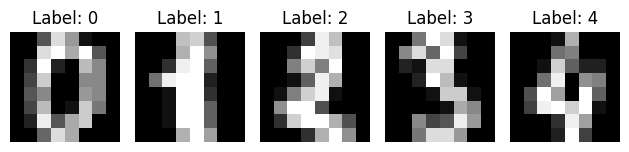
\includegraphics[width=.9\textwidth]{img/digits-vis.png}
    \caption[Five samples from the Digits dataset]{Five $8 \times 8$ samples from the Digits dataset with brightness levels from $0$ to $16$. Correct labels are shown above.}
    \label{fig:digits-vis}
\end{figure}

\paragraph{Preprocessing and input format}
This task involves multiclass classification ($y$: $[0,1,\dots,9]$). Because the input vectors contain features with multiple possible values, they must be transformed into a binary format compatible with the Tsetlin Machine. We achieved this using Scikit-learn's \texttt{OneHotEncoder}, which expanded the feature set from $X$: $(1797, 64)$ with values in $[0,1,\dots,16]$ to $X$: $(1797, 890)$ with binary values $[0,1]$. The data was divided using a typical $80\%$ training and $20\%$ testing split while maintaining class proportions.

\paragraph{Model hyperparameters}
Similar to the Noisy-XOR evaluation, we maintained default parameters while only modifying the \texttt{GridSearchCV} space for our classifier, as shown in Table~\ref{tab:digits-params}. Given the significantly higher number of features in this dataset, the parameter search determined that increasing the number of clauses to $1500$ was beneficial for performance.

\paragraph{Results and comparison}
The results summarized in Table~\ref{tab:digits-results} demonstrate that Tsetlin Machine models can handle more complex datasets. However, because the input format is restricted to binary, the models require a higher number of clauses to capture relevant patterns. This requirement leads to an increase in both time and memory consumption compared to other models. These findings suggest that the binary preprocessing required for TMs may not be ideal for high-dimensional image recognition tasks. Regardless, our implementation maintained accuracy levels comparable to the \GreenTsetlinName library, likely confirming the correctness of our implementation. Slightly longer training and prediction time are likely the result of \LibraryName not implementing vectorization, as decided in the design (see Section~\ref{sec:design}).

\begin{table}[!htbp]
\centering
\caption[Digits hyperparameters]{Hyperparameters and \texttt{GridSearchCV} search spaces for the Digits dataset. The table lists only parameters that differ from model defaults; for \texttt{GridSearchCV} the best-performing configuration is indicated in \texttt{\textbf{\underline{bold}}}\label{tab:digits-params}.}
\begin{tabularx}{\textwidth}{@{}l L@{}} \toprule
    \textbf{Model} & \textbf{Modified Parameters} \\ \midrule \midrule
    \texttt{Logistic Regression} & \texttt{max\_iter=1000} \\ \midrule
    \texttt{Decision Tree} & \texttt{---} \\ \midrule
    \texttt{Random Forest} & \texttt{---} \\ \midrule
    \texttt{MLP} & \texttt{max\_iter=1000, solver="lbfgs"} \\ \midrule
    \texttt{SVC} & \texttt{---} \\ \midrule
    \texttt{Linear SVC} & \texttt{dual="auto"} \\ \midrule
    \texttt{K-Nearest Neighbors} & \texttt{---} \\ \midrule
    \texttt{Gaussian Naive Bayes} & \texttt{---} \\ \midrule
    \texttt{Gradient Boosting} & \texttt{---} \\ \midrule
    \texttt{LightGBM} & \texttt{---} \\ \midrule
    \texttt{GridSearch Random Forest} & \texttt{n\_estimators: [50, 100, \textbf{\underline{200}}], max\_depth: [None, 10, 20, \textbf{\underline{30}}], min\_samples\_split: [\textbf{\underline{2}}, 5, 10]} \\ \midrule
    \texttt{GridSearch MLP} & \texttt{hidden\_layer\_sizes: [(50,), \textbf{\underline{(100,)}}, (50, 50)], activation: ["relu", \textbf{\underline{"tanh"}}], alpha: [0.0001, 0.001, \textbf{\underline{0.01}}]} \\ \midrule \midrule
    \texttt{Green Tsetlin} & \texttt{---}\\ \midrule
    \texttt{Green Tsetlin Sparse} & \texttt{---} \\ \midrule
    \texttt{C Tsetlin} & \texttt{---} \\ \midrule
    \texttt{GridSearch C Tsetlin} & \texttt{boost\_true\_positive\_feedback: [\textbf{\underline{False}}, True], num\_clauses: [500, 1000, \textbf{\underline{1500}}], s: [\textbf{\underline{3}}, 9]} \\ \midrule
    \texttt{C Tsetlin Sparse} & \texttt{---} \\ \midrule
    \texttt{GridSearch C Tsetlin Sparse} & \texttt{boost\_true\_positive\_feedback: [\textbf{\underline{False}}, True], num\_clauses: [64, 125, 500, \textbf{\underline{1000}}], s: [3, \textbf{\underline{9}}]} \\ \bottomrule
\end{tabularx}
\end{table}

\begin{table}[!htbp]
\centering
\setlength{\tabcolsep}{4pt}
\renewcommand{\arraystretch}{0.85}
\setlength{\aboverulesep}{2pt}
\setlength{\belowrulesep}{2pt}
\caption[Digits dataset benchmark results]{Benchmark results for the Digits dataset (evaluated on the Host (PC) environment). Model sizes are estimated based on internal data structures for Tsetlin-based models and via \texttt{pickle} exports for standard models, requiring caution when comparing directly. The best results are indicated in \texttt{\textbf{\underline{bold}}}\label{tab:digits-results}.}
\begin{tabularx}{\textwidth}{@{}l c c c c c r@{}} \toprule
    \textbf{\makecell[l]{Model}} & \textbf{\makecell[l]{Train\\Acc.}} & \textbf{\makecell[l]{Test\\Acc.}} & \textbf{\makecell[l]{Train\\Time (s)}} & \textbf{\makecell[l]{Train\\Pred.\\Time (s)}} & \textbf{\makecell[l]{Test\\Pred.\\Time (s)}} & \textbf{\makecell[l]{Model\\Size (B)}} \\ \midrule
    \texttt{\makecell[l]{Logistic Regression}} & \texttt{\textbf{\underline{1.0000}}} & \texttt{0.9528} & \texttt{1.5764} & \texttt{\textbf{\underline{0.0035}}} & \texttt{0.0042} & \texttt{84,514} \\
    \texttt{\makecell[l]{Decision Tree}} & \texttt{\textbf{\underline{1.0000}}} & \texttt{0.7833} & \texttt{0.0472} & \texttt{0.0038} & \texttt{\textbf{\underline{0.0024}}} & \texttt{\textbf{\underline{59,928}}} \\
    \texttt{\makecell[l]{Random Forest}} & \texttt{\textbf{\underline{1.0000}}} & \texttt{0.9444} & \texttt{0.2000} & \texttt{0.0159} & \texttt{0.0068} & \texttt{9,855,780} \\
    \texttt{\makecell[l]{MLP}} & \texttt{\textbf{\underline{1.0000}}} & \texttt{0.9306} & \texttt{4.5576} & \texttt{0.0226} & \texttt{0.0338} & \texttt{1,461,199} \\
    \texttt{\makecell[l]{SVC}} & \texttt{0.9965} & \texttt{\textbf{\underline{0.9583}}} & \texttt{0.2974} & \texttt{0.3944} & \texttt{0.1206} & \texttt{9,585,426} \\
    \texttt{\makecell[l]{Linear SVC}} & \texttt{\textbf{\underline{1.0000}}} & \texttt{0.9472} & \texttt{0.1006} & \texttt{0.0137} & \texttt{0.0068} & \texttt{84,395} \\
    \texttt{\makecell[l]{K-Nearest Neighbors}} & \texttt{0.9088} & \texttt{0.8667} & \texttt{\textbf{\underline{0.0028}}} & \texttt{0.0679} & \texttt{0.0101} & \texttt{10,256,123} \\
    \texttt{\makecell[l]{Gaussian Naive Bayes}} & \texttt{0.9666} & \texttt{0.8278} & \texttt{0.0062} & \texttt{0.0219} & \texttt{0.0052} & \texttt{155,647} \\
    \texttt{\makecell[l]{Gradient Boosting}} & \texttt{\textbf{\underline{1.0000}}} & \texttt{0.9139} & \texttt{9.5533} & \texttt{0.0150} & \texttt{0.0053} & \texttt{1,359,941} \\
    \texttt{\makecell[l]{LightGBM}} & \texttt{\textbf{\underline{1.0000}}} & \texttt{0.9472} & \texttt{0.6413} & \texttt{0.0092} & \texttt{0.0031} & \texttt{3,124,964} \\
    \texttt{\makecell[l]{GS Random Forest}} & \texttt{\textbf{\underline{1.0000}}} & \texttt{0.9444} & \texttt{5.6181} & \texttt{0.0347} & \texttt{0.0139} & \texttt{19,661,484} \\
    \texttt{\makecell[l]{GS MLP}} & \texttt{\textbf{\underline{1.0000}}} & \texttt{0.9361} & \texttt{8.0691} & \texttt{0.0346} & \texttt{0.0080} & \texttt{1,465,209} \\ \midrule
    \texttt{\makecell[l]{Green Tsetlin}} & \texttt{0.9923} & \texttt{0.9222} & \texttt{1.8070} & \texttt{0.0181} & \texttt{0.0063} & \texttt{1,794,040} \\
    \texttt{\makecell[l]{Green Tsetlin Sparse}} & \texttt{0.9402} & \texttt{0.8889} & \texttt{16.0517} & \texttt{0.0113} & \texttt{0.0042} & \texttt{822,040} \\
    \texttt{\makecell[l]{C Tsetlin}} & \texttt{0.9882} & \texttt{0.9222} & \texttt{18.6141} & \texttt{0.7369} & \texttt{0.1846} & \texttt{1,831,040} \\
    \texttt{\makecell[l]{GS C Tsetlin}} & \texttt{0.9937} & \texttt{0.9139} & \texttt{121.3198} & \texttt{1.0595} & \texttt{0.2674} & \texttt{2,746,540} \\
    \texttt{\makecell[l]{C Tsetlin Sparse}} & \texttt{0.6715} & \texttt{0.5972} & \texttt{21.0368} & \texttt{0.3977} & \texttt{0.1014} & \texttt{970,992} \\
    \texttt{\makecell[l]{GS C Tsetlin Sparse}} & \texttt{0.8045} & \texttt{0.7083} & \texttt{49.0949} & \texttt{0.3634} & \texttt{0.0939} & \texttt{967,712} \\ \bottomrule
\end{tabularx}
\end{table}

\clearpage
\section{Fashion-MNIST Dataset}
The Fashion-MNIST dataset~\cite{xiao2017/online} is a popular image classification task developed as a drop-in replacement for the original MNIST dataset. We utilized this dataset to test the performance limits and scaling capabilities of the Tsetlin Machine, as it is more difficult compared to the Digits dataset. This evaluation is conducted primarily for research purposes as we do not expect our implementation to be used in this types of task otherwise.

\paragraph{Dataset and problem representation}
The dataset consists of $70000$ grayscale images of Zalando's clothing articles. Each example is a $28 \times 28$ pixel image (brightness levels $0$-$255$) associated with one of the $10$ classes. Sample images from the dataset are illustrated in Figure~\ref{fig:fmnist-vis}.

\begin{figure}[!htbp]
    \centering
    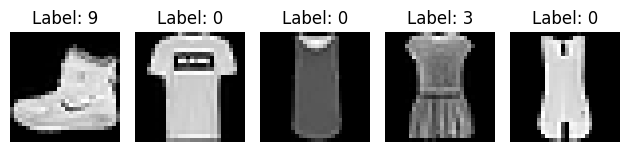
\includegraphics[width=.9\textwidth]{img/fmnist-vis.png}
    \caption[Five samples from the Fashion-MNIST dataset]{Five $28 \times 28$ samples from the Fashion-MNIST dataset with brightness levels from $0$ to $255$ before preprocessing. Correct labels are shown above.}
    \label{fig:fmnist-vis}
\end{figure}

\paragraph{Preprocessing and input format}
To prepare the data for the TM, we selected a subset consisting of the first $10000$ samples. The pixel values were normalized using the division by $16$ and cast to unsigned $8$-bit integers. The original resolution was down-sampled to $14 \times 14$ by selecting every second pixel in both dimensions. These images were then flattened into vectors of $196$ features. Since TMs require binary input, these features were transformed using Scikit-learn's \texttt{OneHotEncoder} with a maximum of $8$ categories. This process transformed the input dimensionality from $X$: $(10000, 784)$ with values in $[0,1,\dots,255]$ to $X$: $(10000, 1555)$ binary features. Finally, the data was divided into $80\%$ training and $20\%$ testing sets while maintaining the class proportions.

\paragraph{Model hyperparameters}
Due to the significant increase in training times with this dataset, we restricted the baseline models only to the Support Vector Classifier (\texttt{SVC}), which is a common method in image recognition tasks. As shown in Table~\ref{tab:f-mnist-params}, all the models evaluated were kept at their default parameter values.

\begin{table}[!htbp]
\centering
\caption[Fashion-MNIST hyperparameters]{Hyperparameters for the Fashion-MNIST dataset. The table lists only parameters that differ from model defaults\label{tab:f-mnist-params}.}
\begin{tabularx}{\textwidth}{@{}l L@{}} \toprule
    \textbf{Model} & \textbf{Modified Parameters} \\ \midrule \midrule
    \texttt{SVC} & \texttt{---} \\ \midrule \midrule
    \texttt{Green Tsetlin} & \texttt{---} \\ \midrule
    \texttt{Green Tsetlin Sparse} & \texttt{---} \\ \midrule
    \texttt{C Tsetlin} & \texttt{---} \\ \midrule
    \texttt{C Tsetlin Sparse} & \texttt{---} \\ \bottomrule
\end{tabularx}
\end{table}

\paragraph{Results and comparison}
The results in Table~\ref{tab:f-mnist-results} indicate that this dataset contains too many features for the current binary approach to TMs to remain efficient. This reveals a limitation in scaling, as all processing times increase significantly. Although both training and testing accuracy were lower than those of the \texttt{SVC}, prediction times for TM-based models remained faster. In particular, our implementation took significantly longer processing times than the \GreenTsetlinName library across all metrics. These findings suggest that the increase in dimensionality and the number of training samples creates performance bottlenecks that are more pronounced in our current implementation than in existing third-party libraries, likely because \LibraryName does not implement vectorization, as decided in the design (see Section~\ref{sec:design}).

\begin{table}[!htbp]
\centering
\setlength{\tabcolsep}{4pt}
\renewcommand{\arraystretch}{0.85}
\setlength{\aboverulesep}{2pt}
\setlength{\belowrulesep}{2pt}
\caption[Fashion-MNIST benchmark results]{Benchmark results for the Fashion-MNIST dataset (evaluated on the Host (PC) environment). Model sizes are estimated based on internal data structures for Tsetlin-based models and via \texttt{pickle} exports for standard models, requiring caution when comparing directly. The best results are indicated in \texttt{\textbf{\underline{bold}}}\label{tab:f-mnist-results}.}
\begin{tabularx}{\textwidth}{@{}l c c c c c r@{}} \toprule
    \textbf{\makecell[l]{Model}} & \textbf{\makecell[l]{Train\\Acc.}} & \textbf{\makecell[l]{Test\\Acc.}} & \textbf{\makecell[l]{Train\\Time (s)}} & \textbf{\makecell[l]{Train\\Pred.\\Time (s)}} & \textbf{\makecell[l]{Test\\Pred.\\Time (s)}} & \textbf{\makecell[l]{Model\\Size (B)}} \\ \midrule
    \texttt{\makecell[l]{SVC}} & \texttt{\textbf{\underline{0.9329}}} & \texttt{\textbf{\underline{0.8260}}} & \texttt{\textbf{\underline{8.3000}}} & \texttt{32.5356} & \texttt{8.2058} & \texttt{66,885,009} \\ \midrule
    \texttt{\makecell[l]{Green Tsetlin}} & \texttt{0.8053} & \texttt{0.7785} & \texttt{15.9906} & \texttt{\textbf{\underline{0.0475}}} & \texttt{\textbf{\underline{0.0136}}} & \texttt{3,124,040} \\
    \texttt{\makecell[l]{Green Tsetlin Sparse}} & \texttt{0.6094} & \texttt{0.5965} & \texttt{201.6389} & \texttt{0.0518} & \texttt{0.0151} & \texttt{\textbf{\underline{822,040}}} \\
    \texttt{\makecell[l]{C Tsetlin}} & \texttt{0.7600} & \texttt{0.7320} & \texttt{209.8398} & \texttt{6.5704} & \texttt{1.6151} & \texttt{3,161,040} \\
    \texttt{\makecell[l]{C Tsetlin Sparse}} & \texttt{0.5821} & \texttt{0.5810} & \texttt{633.4991} & \texttt{3.1626} & \texttt{0.7933} & \texttt{1,271,776} \\ \bottomrule
\end{tabularx}
\end{table}

\clearpage
\section{Incremental Noisy-XOR Learning}
The performance of Tsetlin Machines is highly sensitive to hyperparameter selection, which is often counter-intuitive. This marks the importance of performing an optimal configuration search using tools such as Grid Search. In this section, we evaluate the learning behavior of our model across sequential data batches to understand how specific impact incremental learning.

The training and testing accuracy curves per batch are illustrated in Figure~\ref{fig:noisy-xor-grid}. A comparison between models with different clause counts demonstrated that using $1000$ clauses allows the model to learn faster and achieve higher stability compared to using only $100$ clauses. This behavior shown in Figures~\ref{fig:noisy-xor-100-1}~and~\ref{fig:noisy-xor-1000-1} suggests that a larger pool of clauses may allow individual units to ``catch up'' to patterns more quickly.

The experimental results presented in Figures~\ref{fig:noisy-xor-1000-1}~and~\ref{fig:noisy-xor-1000-10} indicate that while increasing the number of epochs per batch improves accuracy on the current batch, it leads to the degradation of previously learned patterns, resulting in worse overall performance. This drop in accuracy is likely a consequence of the TM's internal forgetting mechanism during feedback processing. This presents a challenge for incremental learning, where maintaining a balance between retaining knowledge and memorizing new patterns is crucial.

\begin{figure}[!htbp]
    \centering
    % Row 1, Left
    \begin{subfigure}{0.49\textwidth}
        \centering
        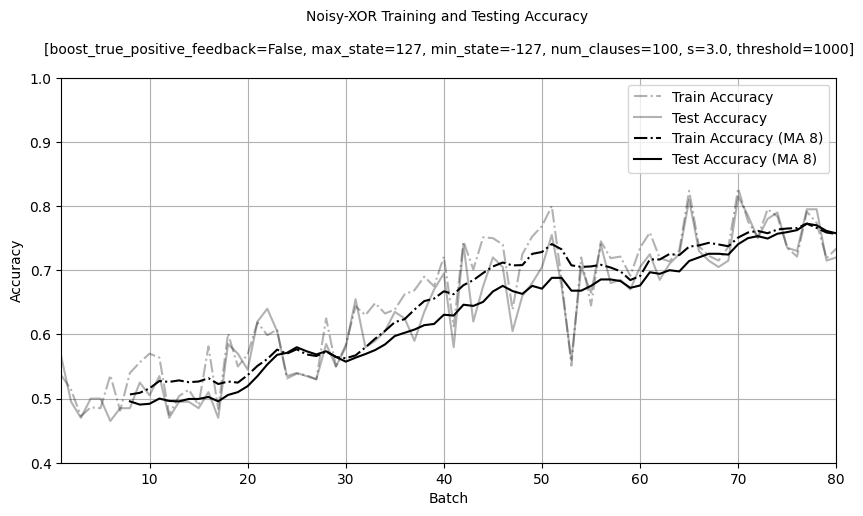
\includegraphics[width=\textwidth]{img/noisy-xor-100-clauses-1-epoch-per-batch.png}
        \caption{100 clauses, 1 epoch per batch}
        \label{fig:noisy-xor-100-1}
    \end{subfigure}
    \hfill
    % Row 1, Right
    \begin{subfigure}{0.49\textwidth}
        \centering
        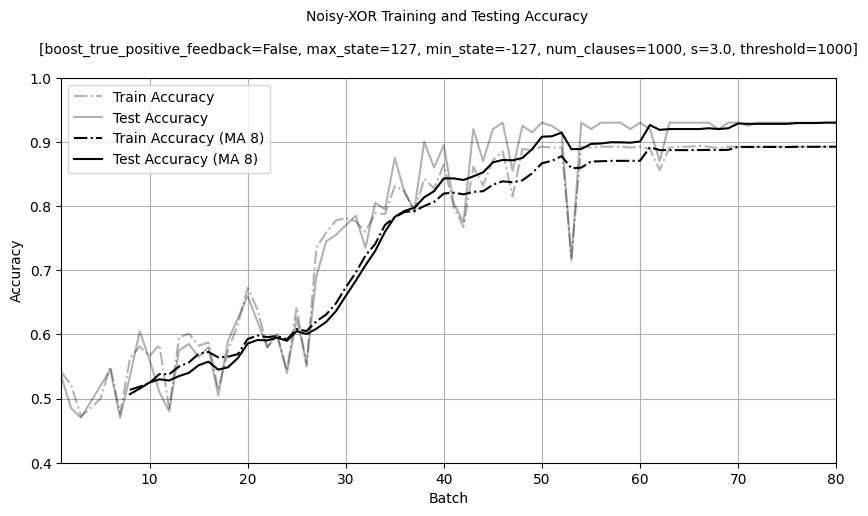
\includegraphics[width=\textwidth]{img/noisy-xor-1000-clauses-1-epoch-per-batch.png}
        \caption{1000 clauses, 1 epoch per batch}
        \label{fig:noisy-xor-1000-1}
    \end{subfigure}

    \vspace{1em}

    % Row 2, Left
    \begin{subfigure}{0.49\textwidth}
        \centering
        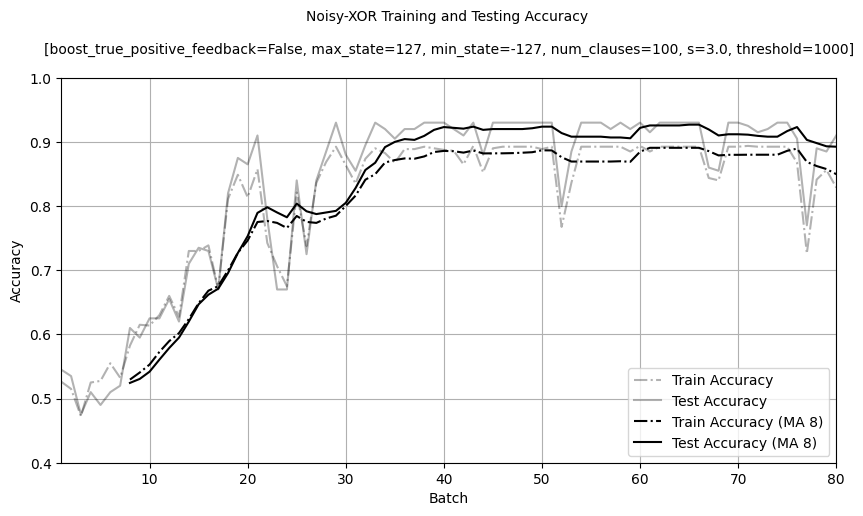
\includegraphics[width=\textwidth]{img/noisy-xor-100-clauses-10-epoch-per-batch.png}
        \caption{100 clauses, 10 epochs per batch}
        \label{fig:noisy-xor-100-10}
    \end{subfigure}
    \hfill
    % Row 2, Right
    \begin{subfigure}{0.49\textwidth}
        \centering
        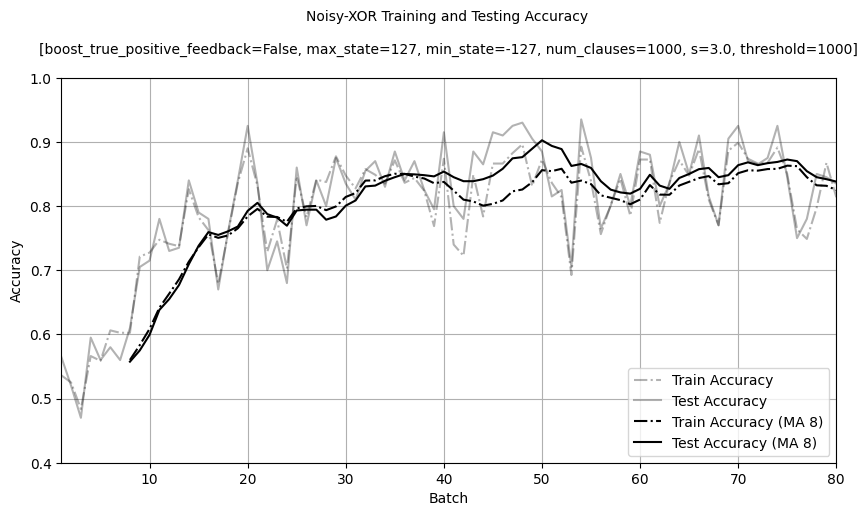
\includegraphics[width=\textwidth]{img/noisy-xor-1000-clauses-10-epoch-per-batch.png}
        \caption{1000 clauses, 10 epochs per batch}
        \label{fig:noisy-xor-1000-10}
    \end{subfigure}

    \caption[Train and test accuracy per batch on the Noisy-XOR]{Train accuracy (dash-dot line) and test accuracy (solid line) per batch for the Noisy-XOR dataset. The evaluation tracks progress over 80 batches of 10 samples each.}
    \label{fig:noisy-xor-grid}
\end{figure}

\clearpage
\section{Embedded Noisy-XOR Benchmarks}
We demonstrated the capability of our implementation by running the minimal version of the core C library on resource-constrained hardware. As a target platform, we chose the Raspberry Pi Pico development board due to its popularity and software support, specifically the Pico-SDK~\cite{pico-sdk}. The platform is powered by the RP2040 microcontroller chip, featuring a dual-core Arm Cortex-M0+ processor clocked at 133 MHz, 264 KB of SRAM and 2 MB of on-board flash memory.

We conducted benchmarks on the Noisy-XOR dataset similar to those performed in Python but using a wider range of configurations. Selected tests were performed on a desktop PC running Ubuntu OS in cases where the models exceeded the hardware performance limits of the Raspberry Pi Pico or where peak memory statistics were unavailable. The results are detailed in Table~\ref{tab:noisy-xor-pi-pico}, with values gathered from the Ubuntu environment marked with a \textbf{(U)} prefix.

The analysis reveals several important characteristics:
\begin{compactitem}
    \item Tsetlin Machine memory usage (\textbf{TMM}) is directly proportional only to the number of clauses.
    \item Training time (\textbf{TRT}) is proportional to the number of clauses, samples, and epochs.
    \item Evaluation time (\textbf{EVT}) is also proportional to the number of clauses, and samples.
    \item Other hyperparameters than mentioned above have a relatively small impact on performance when set to values close to established model defaults.
    \item Accurately measuring peak memory usage (\textbf{PMU}) proved difficult in the Ubuntu environment due to system overhead.
\end{compactitem}

As shown in Table~\ref{tab:noisy-xor-pi-pico}, our implementation remains highly usable on embedded hardware. For example, configurations \textbf{9} and \textbf{10} achieve accuracy levels close to the theoretical maximum (counting for the $10\%$ added noise). We can observe a clear trade-off: using more epochs and fewer clauses (Configuration \textbf{10}) results in a longer training time but a smaller memory footprint and faster prediction speeds, which is ideal for pretrained models. In contrast, using a single epoch with more clauses (Configuration \textbf{9}) allows faster on-device learning at the cost of increased model size and slower evaluation.

\begin{sidewaystable}[!htbp]
\centering
\scriptsize
\setlength{\tabcolsep}{2.5pt}
\caption[Noisy-XOR performance on Raspberry Pi Pico]{Noisy-XOR results on Raspberry Pi Pico and Ubuntu Desktop (the Host (PC) environment), testing how hyperparameters affect accuracy and execution time. Peak RAM usage was calculated on the Ubuntu Desktop and includes system overhead. Due to hardware performance limits, configurations exceeding the 1000 clauses were benchmarked only on Ubuntu (marked with \textbf{(U)} prefix)\label{tab:noisy-xor-pi-pico}.}
\begin{tabular}{@{}r r r r r r r r r r r r r r r r r r r r@{}} \toprule
    \textbf{N} & \textbf{SAM} & \textbf{CLS} & \textbf{THR} & \textbf{LIT} & \textbf{CLU} & \textbf{MXS} & \textbf{MNS} & \textbf{BST} & \textbf{SNS} & \textbf{EPC} & \textbf{TRT} & \textbf{EVT} & \textbf{COP} & \textbf{TOP} & \textbf{ACC} & \textbf{TMM} & \textbf{DSM} & \textbf{PMU} \\ \midrule
    1 & 1000 & 2 & 1000 & 16 & 1000 & 127 & -127 & 0 & 3.0 & 1 & 24.73 & 0.88 & 183 & 200 & 0.92 & 36.21 & 19.53 & \textbf{(U)}1728.0 \\
    2 & 1000 & 2 & 1000 & 16 & 1000 & 127 & -127 & 0 & 3.0 & 2 & 41.30 & 0.87 & 183 & 200 & 0.92 & 36.21 & 19.53 & \textbf{(U)}1728.0 \\
    3 & 1000 & 2 & 1000 & 16 & 1000 & 127 & -127 & 0 & 3.0 & 4 & 72.51 & 0.88 & 183 & 200 & 0.92 & 36.21 & 19.53 & \textbf{(U)}1728.0 \\
    4 & 1000 & 2 & 1000 & 16 & 1000 & 63 & -63 & 0 & 3.0 & 1 & 24.73 & 0.88 & 183 & 200 & 0.92 & 36.21 & 19.53 & \textbf{(U)}1728.0 \\
    5 & 1000 & 2 & 1000 & 16 & 1000 & 31 & -31 & 0 & 3.0 & 1 & 24.73 & 0.88 & 183 & 200 & 0.92 & 36.21 & 19.53 & \textbf{(U)}1728.0 \\
    6 & 1000 & 2 & 1000 & 16 & 1000 & 15 & -15 & 0 & 3.0 & 1 & 24.51 & 0.86 & 183 & 200 & 0.92 & 36.21 & 19.53 & \textbf{(U)}1728.0 \\
    7 & 1000 & 2 & 1000 & 16 & 500 & 127 & -127 & 0 & 3.0 & 1 & 12.92 & 0.40 & 183 & 200 & 0.92 & 18.15 & 19.53 & \textbf{(U)}1728.0 \\
    8 & 1000 & 2 & 1000 & 16 & 250 & 127 & -127 & 0 & 3.0 & 1 & 6.79 & 0.21 & 183 & 200 & 0.92 & 9.12 & 19.53 & \textbf{(U)}1728.0 \\
    \textbf{\underline{9}} & 1000 & 2 & 1000 & 16 & 125 & 127 & -127 & 0 & 3.0 & 1 & 3.54 & 0.10 & 183 & 200 & 0.92 & 4.6 & 19.53 & \textbf{(U)}1728.0 \\
    \textbf{\underline{10}} & 1000 & 2 & 1000 & 16 & 64 & 127 & -127 & 0 & 3.0 & 10 & 11.93 & 0.05 & 183 & 200 & 0.92 & 2.39 & 19.53 & \textbf{(U)}1728.0 \\
    11 & 1000 & 2 & 1000 & 16 & 1000 & 127 & -127 & 0 & 3.0 & 10 & 163.19 & 0.89 & 182 & 200 & 0.91 & 36.21 & 19.53 & \textbf{(U)}1728.0 \\
    12 & 1000 & 2 & 500 & 16 & 1000 & 127 & -127 & 0 & 3.0 & 1 & 22.98 & 0.87 & 182 & 200 & 0.91 & 36.21 & 19.53 & \textbf{(U)}1728.0 \\
    13 & 1000 & 2 & 1000 & 16 & 1000 & 127 & -127 & 1 & 3.0 & 1 & 24.53 & 0.82 & 181 & 200 & 0.91 & 36.21 & 19.53 & \textbf{(U)}1728.0 \\
    14 & 1000 & 2 & 250 & 16 & 1000 & 127 & -127 & 0 & 3.0 & 1 & 22.58 & 0.89 & 180 & 200 & 0.9 & 36.21 & 19.53 & \textbf{(U)}1728.0 \\
    15 & 1000 & 2 & 1000 & 16 & 1000 & 127 & -127 & 0 & 6.0 & 1 & 26.33 & 0.67 & 179 & 200 & 0.9 & 36.21 & 19.53 & \textbf{(U)}1728.0 \\
    16 & 1000 & 2 & 32 & 16 & 1000 & 127 & -127 & 0 & 3.0 & 1 & 21.30 & 0.87 & 179 & 200 & 0.9 & 36.21 & 19.53 & \textbf{(U)}1728.0 \\
    17 & 250 & 2 & 1000 & 16 & 1000 & 127 & -127 & 0 & 3.0 & 10 & 47.14 & 0.22 & 44 & 50 & 0.88 & 36.21 & 4.88 & \textbf{(U)}1728.0 \\
    18 & 1000 & 2 & 125 & 16 & 1000 & 127 & -127 & 0 & 3.0 & 1 & 21.54 & 0.88 & 173 & 200 & 0.87 & 36.21 & 19.53 & \textbf{(U)}1728.0 \\
    19 & 1000 & 2 & 64 & 16 & 1000 & 127 & -127 & 0 & 3.0 & 1 & 21.03 & 0.88 & 170 & 200 & 0.85 & 36.21 & 19.53 & \textbf{(U)}1728.0 \\
    20 & 1000 & 2 & 32 & 16 & 500 & 127 & -127 & 0 & 3.0 & 1 & 10.87 & 0.44 & 168 & 200 & 0.84 & 18.15 & 19.53 & \textbf{(U)}1728.0 \\
    21 & 1000 & 2 & 32 & 16 & 500 & 127 & -127 & 0 & 3.0 & 10 & 79.82 & 0.46 & 166 & 200 & 0.83 & 18.15 & 19.53 & \textbf{(U)}1728.0 \\
    22 & 1000 & 2 & 1000 & 16 & 1000 & 7 & -7 & 0 & 3.0 & 1 & 27.17 & 0.81 & 165 & 200 & 0.83 & 36.21 & 19.53 & \textbf{(U)}1728.0 \\
    23 & 1000 & 2 & 1000 & 16 & 64 & 127 & -127 & 0 & 3.0 & 1 & 1.85 & 0.05 & 162 & 200 & 0.81 & 2.39 & 19.53 & \textbf{(U)}1728.0 \\
    24 & 1000 & 2 & 16 & 16 & 1000 & 127 & -127 & 0 & 3.0 & 1 & 21.27 & 0.85 & 161 & 200 & 0.81 & 36.21 & 19.53 & \textbf{(U)}1728.0 \\
    25 & 500 & 2 & 1000 & 16 & 1000 & 127 & -127 & 0 & 3.0 & 1 & 36.21 & 0.44 & 80 & 100 & 0.8 & 36.21 & 9.77 & \textbf{(U)}1728.0 \\
    26 & 1000 & 2 & 32 & 16 & 500 & 127 & -127 & 1 & 3.0 & 1 & 10.74 & 0.42 & 150 & 200 & 0.75 & 18.15 & 19.53 & \textbf{(U)}1728.0 \\
    27 & 1000 & 2 & 1000 & 16 & 64 & 127 & -127 & 1 & 3.0 & 1 & 1.79 & 0.05 & 142 & 200 & 0.71 & 2.39 & 19.53 & \textbf{(U)}1728.0 \\
    28 & 1000 & 2 & 1000 & 16 & 1000 & 127 & -127 & 0 & 1.5 & 1 & 30.84 & 1.15 & 124 & 200 & 0.62 & 36.21 & 19.53 & \textbf{(U)}1728.0 \\
    29 & 250 & 2 & 1000 & 16 & 1000 & 127 & -127 & 0 & 3.0 & 1 & 7.21 & 0.22 & 27 & 50 & 0.54 & 36.21 & 4.88 & \textbf{(U)}1728.0 \\
    30 & 1000 & 2 & 1000 & 16 & 1000 & 3 & -3 & 0 & 3.0 & 1 & 28.43 & 0.73 & 100 & 200 & 0.5 & 36.21 & 19.53 & \textbf{(U)}1728.0 \\
    31 & 1000 & 2 & 1000 & 16 & 10000 & 127 & -127 & 0 & 3.0 & 1 & \textbf{(U)}1.16 & \textbf{(U)}0.11 & 172 & 200 & 0.86 & 361.45 & 19.53 & \textbf{(U)}2112.0 \\
    32 & 1000 & 2 & 1000 & 16 & 100000 & 127 & -127 & 0 & 3.0 & 1 & \textbf{(U)}11.61 & \textbf{(U)}1.17 & 167 & 200 & 0.84 & 3613.4 & 19.53 & \textbf{(U)}5376.0 \\
    33 & 1000 & 2 & 1000 & 16 & 200000 & 127 & -127 & 0 & 3.0 & 1 & \textbf{(U)}23.00 & \textbf{(U)}2.32 & 165 & 200 & 0.83 & 7226.68 & 19.53 & \textbf{(U)}8832.0 \\ \bottomrule
\end{tabular}
\vspace{1ex}
\begin{flushleft}
\textbf{Legend:} 
\textbf{N}:~Configuration Number,
\textbf{SAM}:~Number of Samples, 
\textbf{CLS}:~Number of Classes, 
\textbf{THR}:~Threshold, 
\textbf{LIT}:~Number of Literals, 
\textbf{CLU}:~Number of Clauses, 
\textbf{MXS}:~Maximum State,
\textbf{MNS}:~Minimum State,
\textbf{BST}:~Boost True Positive Feedback,
\textbf{SNS}:~Learning Sensitivity (s),
\textbf{EPC}:~Training Epochs,
\textbf{TRT}:~Training Time [s],
\textbf{EVT}:~Evaluation Time [s],
\textbf{COP}:~Correct Predictions,
\textbf{TOP}:~Total Predictions,
\textbf{ACC}:~Accuracy,
\textbf{TMM}:~TM Memory Usage [KB],
\textbf{DSM}:~Dataset Memory Usage (\texttt{static}) [KB],
\textbf{PMU}:~Peak Memory Usage on Ubuntu Desktop [KB]
\end{flushleft}
\end{sidewaystable}

\clearpage
\section{Summary}
The initial evaluation of our Tsetlin Machine implementations shows potential, especially for resource-limited environments dealing with not overly high-dimensional data. We observed the impact of hyperparameters, mainly number of clauses and training epochs, making it essential to tune them for each task. We observed the mechanism inside TM designed to prevent overfitting, creating a challenge in incremental learning, where the balance between retaining old knowledge and memorizing new patterns is crucial. Furthermore, benchmarking was complicated due to the \GreenTsetlinName library design, which includes some undocumented optimizations (e.g. \texttt{literal\_budget} parameter that is not properly described).